% A paper that seeks to provide a formal definition of proportionality, typeset in LaTeX
\documentclass{article}
\usepackage{graphicx}
\usepackage{tikz}

\begin{document}

\title{Introduction to \LaTeX{}}
\author{Author's Name}

\maketitle

\begin{abstract}
The abstract text goes here.
\end{abstract}

\section{Introduction}
Here is the text of your introduction.d

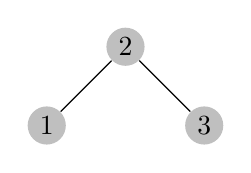
\begin{tikzpicture}[shorten >=1pt,->]
  \tikzstyle{vertex}=[circle,fill=black!25,minimum size=12pt,inner sep=2pt]
  \node[vertex] (G_1) at (-1,-1) {1};
  \node[vertex] (G_2) at (0,0)   {2};
  \node[vertex] (G_3) at (1,-1)  {3};
  \draw (G_1) -- (G_2) -- (G_3) -- cycle;
\end{tikzpicture}}

\subsection{Subsection Heading Here}
Write your subsection text here.

\section{Conclusion}
Write your conclusion here.

\end{document}
